Think of a \PJOB{} file as self contained \PHO{} calculation job.
A \PJOB{} file contains all information needed to run the job.
The only extra part is \PHO{} itself.\bb

This file format was introduced to make the creation and sharing of complex simulation scenarios easier.
A \pjob\ file incorporates all data necessary to run a complex job.
Depending on the actual simulation scenario this may be several \pho\ files, \matlab\ files, \pscript\ files
or some user defined data structures.\bb

\pjob\ files may declare parameters that have to be provided when executing the job.
Also \pjob\ files may have multiple results.
Parameters and results constitute the interface of a concrete \pjob\ file.
Systems such as \PQUEUE{} don't need to know how a \pjob\ is implemented.
The numbers and names of parameters and results is all it needs to know
in order to work with the \pjob{}. 
A \pjob\ file uses XML files to determine what parameters may be provided when executing the job,
what results are created and in which files these results are written. \bb

When running a \pjob\ file \photoss\ writes the simulation results into the executed \pjob\ file.
Already existing results are preserved so a \pjob\ file saves the history of all executions of a job.\bb






\subsection{Creating a \PJOB{} file}
The rest of this section covers the details of the \pjob\ file format.
In order to create a \pjob\ file, you won't need to know all of this if you use the \PJOB-Editor.
See section \ref{section:pjob-editor} for a description of how to create \pjob\ files with the \PJOB-Editor.\bb

If you want to create \pjob\ files programmatically you could either write \pjob\ files yourself
according to the definitions given in this chapter
or you could create all the \pjob file's contents in a separate directory and archive this directory
into a \pjob\ file using the \PJOBCMD\ tool.
See section \ref{section:pjob-cmd} for more information on this.\bb

Either way, you need to know the basics on how to implement a \pjob.
\pjob\ files use \PS{} to enable the user to do user defined actions within an \PJOB{}.
Every \PJOB{} needs to include a main.pscript file that gets executed when \PHO{} runs the job.
In main.pscript, code can be provided that loads and runs a \pho\ file for example.
Before executing the script, \PHO{} changes its current working directory to the resources directory
where the main.pscript file resides.
Also before executing, declared parameters are set to the provided values
(or default values if no values are provided to \PHO{}' command line)
and are made available in the script's context.

For example, if a \PJOB{} file declares a parameter named \textit{length}
and contains a file named \textit{my\_system.pho}
the following main.pscript will run the provided \pho\ file
after setting the value of \textit{length} as the fiber's length:

\lstset{language=JavaScript}
\lstset{backgroundcolor=\color{gray}}
\begin{lstlisting}
sim = Application.openSimulation("my_system.pho");
sim.SMF.length = Application.parameters.length;
sim.run();
\end{lstlisting}

It is the \PJOB{}'s creator's responsibility to assemble a functional \PJOB{} file.
The main.pscript listed above relies on a \textit{my\_system.pho} containing a component named \textit{SMF}
that has a parameter named \textit{length}.
Also it relies on the declaration of a \PJOB{} file parameter named \textit{length}.
If any of these assumptions is not met \PHO{} won't be able to execute and will stop premature
leaving an empty run directory without results.




\subsection{Structure}
\label{pjob:structure}
\pjob\ files are archives containing a particular file structure as depicted in figure \ref{filestructure}.
\begin{figure}[h!]
%\centering
\caption{File structure of a \pjob\ file. \textbf{Bold} entries represent directories.}
\label{filestructure}
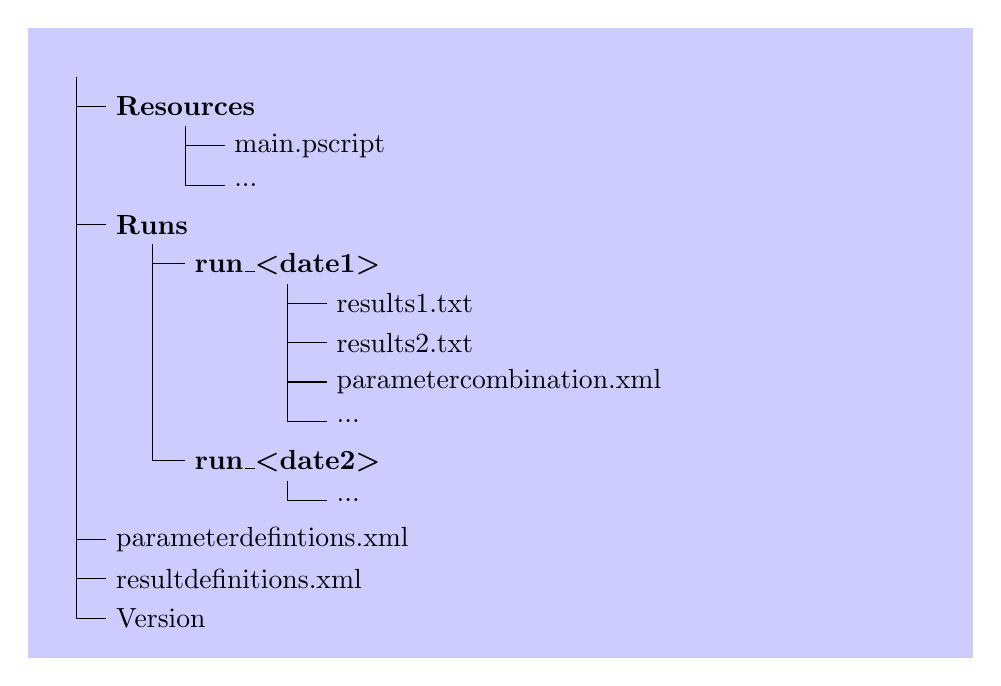
\begin{tikzpicture}
\fill[blue!20] (0,0) rectangle (12cm,-8cm);
\draw (0.5,-0.5) node[anchor=west](root) {\\};
	\draw (1,-1) node[anchor=west,font=\bfseries](Res) {Resources};
		\draw (2.5,-1.5) node[anchor=west](main) {main.pscript};
		\draw (2.5,-2) node[anchor=west] (ResDots){...};
	\draw (1,-2.5) node[anchor=west,font=\bfseries] (Runs) {Runs};
		\draw (2,-3) node[anchor=west,font=\bfseries] (Run1) {run\_\textless date1\textgreater};
			\draw (3.8,-3.5) node[anchor=west](Run1Main) {results1.txt};
			\draw (3.8,-4) node[anchor=west] (Run1Dots) {results2.txt};
			\draw (3.8,-4.5) node[anchor=west](Run1Params) {parametercombination.xml};
			\draw (3.8,-5) node[anchor=west](Run1Results) {...};
		\draw (2,-5.5) node[anchor=west,font=\bfseries] (Run2) {run\_\textless date2\textgreater};
			\draw (3.8,-6) node[anchor=west] (Run2Dots) {...};
	\draw (1,-6.5) node[anchor=west] (Parameterdefinitions) {parameterdefintions.xml};
	\draw (1,-7) node[anchor=west] (Resultdefinitions) {resultdefinitions.xml};
	\draw (1,-7.5) node[anchor=west] (Version) {Version};

\draw (root.south) |- (Res.west);
\draw (root.south) |- (Runs.west);
\draw (root.south) |- (Parameterdefinitions.west);
\draw (root.south) |- (Resultdefinitions.west);
\draw (root.south) |- (Version.west);
\draw (Res.south) |- (main.west);
\draw (Res.south) |- (ResDots.west);
\draw (Runs.south) |- (Run1.west);
\draw (Runs.south) |- (Run2.west);
\draw (Run1.south) |- (Run1Dots.west);
\draw (Run1.south) |- (Run1Main.west);
\draw (Run1.south) |- (Run1Params.west);
\draw (Run1.south) |- (Run1Results.west);
\draw (Run2.south) |- (Run2Dots.west);
\end{tikzpicture}
\end{figure}


The following entries are mandatory:
\begin{itemize}
\item Directory \textit{Resources} containing a file \textit{main.pscript}
\item Directory \textit{Runs} (may be empty)
\item Files \textit{parameterdefintions.xml}, \textit{resultdefinitions.xml} and \textit{Version}
\end{itemize}
The directory \textit{Resources} may contain any number of files or directories of any depth.
\textit{Resources/main.pscript} must be a valid \textsc{PScript} file.
For every (already completed) execution of the job there is a subdirectory in the \textit{Run} directory.
These subdirectories are named \textit{run\_} plus the date of the execution
in the format \textit{YYYYMMDD\_hhmm} (so that lexical sorting makes it easy to find the latest run).

File \textit{Version} contains the \pjob\ file's version as string.
So for the first version this is \textit{``1.0''}. Will be different in future versions of \pjob\ files.

\subsubsection{Underlying archive format}
\label{pjob:archive_format}
\pjob\ files use a self-made binary archive format to concatenate the files contained in a \pjob\ file.
The first 21 bytes are occupied by the file header.
It starts with the 9 byte string \texttt{PJobFile\textbackslash n}
followed by the file's version number represented as a 4 byte little endian integer (TODO: signed or unsigned?).
The header's third and last field is a 8 byte little endian long integer (TODO: signed or unsigned?)
that tells the files last modification date in seconds since the Unix Epoch (00:00:00 UTC on 1 January 1970).

The file's content consists of chunks,
one for every file that is archived in it.
Each chunk itself consists of a chunk header and its content (the file content).
The chunk header's first field is a newline terminated string that represents the filename
associated with this chunk,
including its relative (to this archive), forward slash (\texttt{/})
seperated file path (for example \texttt{Resources/main.pscript}).
The filename is followed by the file's last modification date as a 8 byte little endian long integer,
again representing the number of seconds since the Unix Epoch.
Third and last chunk header field is a 4 byte little endian integer representing
the chunk's body's size in bytes.
This is directly followed by the body that is the file's zlib compressed content.

\begin{figure}[h!]
\caption{\pjob's underlying binary format.}
\label{binary_format}
\begin{tikzpicture}
	\draw (-2,-0.5) node {Header:};
	\draw (0,0) rectangle (4.5,-1) rectangle (6.5,0) rectangle (10.5,-1);
	\draw (2.25, -0.5) node {\texttt{PJobFile\textbackslash n}}
	      (5.5, -0.5) node {version}
	      (8.5, -0.5) node {modification date};
	
    \draw[snake=brace] (0.2,0.2) -- node[above]{9 byte} (4.3,0.2)
                       (4.7,0.2) -- node[above]{4 byte} (6.3,0.2)
                       (6.7,0.2) -- node[above]{8 byte} (10.3,0.2);

    \draw (-2,-2.5) node {Chunk:};
    \draw (0,-2) rectangle (4.5,-3) rectangle (8.5,-2) rectangle (10.5,-3) rectangle (0,-5);
	\draw (2.25, -2.5) node {file path (\textbackslash n terminated)}
	      (6.5, -2.5) node {modification date}
	      (9.5, -2.5) node {size}
	      (5.25, -4) node {zlib compressed file content};
	
	\draw[snake=brace] (0.2,-1.8) -- node[above]{dynamic} (4.3,-1.8)
                       (4.7,-1.8) -- node[above]{8 byte} (8.3,-1.8)
                       (8.7,-1.8) -- node[above]{4 byte} (10.3,-1.8)
                       (10.7,-2.2) -- node[right]{chunk header} (10.7,-2.8)
                       (10.7,-3.2) -- node[right]{chunk body, \textit{size} bytes} (10.7,-4.8);

    \draw (-2,-6.5) node {More chunks..};
\end{tikzpicture}
\end{figure}

This format makes it easy to add files to the archive,
chunks can be appended at the end of the file.
There is no sorting required.
The tree-like file structure is implied by the file names which also include the path
and therefore the directory.
One negligible drawback is that there is no way to have an empty directory.
The file's contents can be scanned by hopping from chunk header to chunk header,
omitting the content.

\subsubsection{Parameters}
\label{pjob:parameters}
A \pjob\ file may declare parameters that can be assigned values to when executing the job with \photoss.
Once declared, these parameteres will be available in the main.pscript's context,
that is the \pjob's script may assume that variables with the parameter's names
have been set before executing the main.pscript.
Furthermore the parameter's values are checked to be within the specified boundaries.

The file \textit{parameterdefinitions.xml} defines which parameters may be provided when executing the job.
This must be consistent with the code in \textit{main.pscript},
i.e. parameters needed by the script must be declared here.
For every parameter a name and a default value has to be provided,
a minimum or maximum value can be provided.
A \textit{parameterdefinitions.xml} file may look like this:
\lstset{language=XML}
\lstset{basicstyle=\color{black},backgroundcolor=\color{gray}}
\begin{lstlisting}
<parameterdefinitions>
	<parameter>
		<name>length</name>
		<defaultValue>100</defaultValue>
	</parameter>
	<parameter>
		<name>power</name>
		<unit>dBm</unit>
		<defaultValue>5</defaultValue>
		<min>1</min>
		<max>15</max>
	</parameter>
</parameterdefinitions>
\end{lstlisting}
A XML Schema Definition for this XML file is provided in the appendix.\bb

When executed a \textit{parametercombination.xml} file is saved in the run directory.
This file contains the information for which parameter values the job was executed.
It is either constructed by \photoss\ according to the default values
provided with the \textit{parameterdefinitions.xml}
or it was passed by the user as an argument in order to run the job with parameter values
differing from the default values.

A \textit{parametercombination.xml} may look like this:
\begin{lstlisting}
<parametercombination>
	<parameter>
		<name>length</name>
		<value>50</value>
	</parameter>
	<parameter>
		<name>power</name>
		<variation>
			<min>3</min>
			<max>7</max>
			<step>1</step>
		</variation>
	</parameter>
</parametercombination>
\end{lstlisting}
Again a XML Schema Definition is provided in the appendix.\bb

On execution parameters are made available to the script.
For every parameter defined in \textit{parameterdefinitions.xml}
the global Property
\lstset{language=JavaScript}
\begin{lstlisting}
Application.parameters
\end{lstlisting}
will have a property named as the corresponding parameter.
These properties have subproperties \textit{isVariation()}
and either \textit{value} or \textit{min}, \textit{max}, \textit{step} and \textit{values}.
So a \textit{main.pscript} according to the example stated above may look like this:
\begin{lstlisting}
if(Application.parameters.length.isVariation()){
	for(var i in Application.parameters.length.values)
		...
}else{
	var length = Application.parameters.length.value;
	...
}

if(Application.parameters.power.isVariation()){
	for(var i in Application.parameters.length.values)
		...
}else{
	var power = Application.parameters.power.value;
	...
}
\end{lstlisting}



\subsubsection{Results}
\label{pjob:results}
All files created on execution reside in the run directory.
Which files are created depends on the code contained in the file \textit{Resources/main.pscript}.
In order to be able to access a job's results without having to know its implementation
the file \textit{resultdefinitions.xml} declares which files contain results
and what format they use.
A \textit{resultdefinitions.xml} declaring one result file which contains two results may look like this:
\lstset{language=XML}
\begin{lstlisting}
<resultdefinitions>
	<resultFile>
		<filename>Results.txt</filename>
		<format>CSV</format>
		<result>
			<name>EOP</name>
		</result>
		<result>
			<name>Q</name>
			<unit>dB</unit>
		</result>
	</resultFile>
</resultdefinitions>
\end{lstlisting}
Allowed format types are \textit{SINGLE\_VALUE} and \textit{CSV}.
\textit{SINGLE\_VALUE} is the format used by \PHO\ component results,
that is only one floating point number as text (i.e. multiple characters)
and nothing else.
Decimal point is ``.''

\textit{CSV} is for \textit{comma separated values} (also called \textit{flat files}) and is the format used by \PHO\ for parameter variation results.
These files consist of rows separated by newline characters.
Each row consists of fields separated by tabulator characters.
The first lines constitute a header (marked with ``\%'') stating the columns names.
Some columns represent varied simulation parameters and some simulation results.
This is indicated by the columns name and is context dependent.
There is one row for each regarded parameter combination.



\subsection{Execution of a \pjob\ file}
When running a \pjob\ file \photoss\ first extracts its contents to a temporary directory.
It then creates a new subdirectory under \textit{Runs}
named \textit{run\_} plus the current date and time
and copies all files and directories from \textit{Resources} to that newly created run directory.
\photoss\ changes its current working directory to that run directory and
executes the \textsc{PScript} file \textit{main.pscript}.
As described above parameters are therefore added to the \textsc{PScript} context before evaluating the script.
After the script has finished execution,
\PHO{} compares all files within the run directory with the files in the resource directory and deletes files
that weren't changed during execution in order to prevent redundancy and \PJOB{} files from becoming too big.
Then the temporary directory
(with the newly created run directory and the results therein)
is written back to the \pjob\ file.


\subsubsection{Providing \PJOB\ parameters on execution}
A \PJOB\ file can be executed by calling \PHO\ with the path to the \PJOB\ file as argument.
\lstset{basicstyle=\color{white},backgroundcolor=\color{black}, language=bash}
\begin{lstlisting}
lucksus:~ nico$ PHOTOSS_cmd Desktop/my_first.pjob
\end{lstlisting}
If no parameter values are given, \PHO\ sets the default values stored with the parameter definition.
Parameter values can be provided by using \PHO's command line switch \textit{--param} (short: \textit{-p})
followed by the parameter's name and a value.
\begin{lstlisting}
lucksus:~ nico$ PHOTOSS_cmd Desktop/my_first.pjob --param length 100
\end{lstlisting}
Multiple parameters are set either by using multiple \textit{--param} switches
\begin{lstlisting}
lucksus:~ nico$ PHOTOSS_cmd Desktop/my_first.pjob -p length 100 -p power 5
\end{lstlisting}
or by using the \textit{--parametercombination} (short: \textit{-c}) switch and providing the path to a parameter combination file
as described in \ref{pjob:parameters} above.
\begin{lstlisting}
lucksus:~ nico$ PHOTOSS_cmd Desktop/my_first.pjob -c Desktop/parametercombination.xml
\end{lstlisting}

\subsubsection{Parameter variations}
\PJOB\ parameters can be set to be varied.
The \PJOB's main.pscript needs to support this, i.e. has to include code that iterates over all variation values, as is shown in \ref{pjob:parameters}.
Variation values can again either be provided via command line, using \PHO's \textit{--param} switch with the syntax described in the \PHO\ application manual
\begin{lstlisting}
lucksus:~ nico$ PHOTOSS_cmd Desktop/my_first.pjob -p length 10:20:1 -p power 5
\end{lstlisting}
or by writing a parameter combination file.
One equivalent to the example above looks like this:
\lstset{language=XML}
\lstset{basicstyle=\color{black},backgroundcolor=\color{gray}}
\begin{lstlisting}
<parametercombination>
	<parameter>
		<name>length</name>
		<variation>
			<min>10</min>
			<max>20</max>
			<step>1</step>
		</variation>
	</parameter>
	<parameter>
		<name>power</name>
		<value>5</value>
	</parameter>
</parametercombination>
\end{lstlisting}

